\documentclass[12pt]{article} %Teckenstorlek 12pt, och format ‘rapport’
\usepackage[utf8]{inputenc}
\usepackage[T1]{fontenc}
\usepackage{amsmath, amsthm, amssymb}
\usepackage[pdftex]{graphicx}
\usepackage{float}
\usepackage{caption}
\usepackage{placeins}
\usepackage{hyperref}
\usepackage{graphicx}
\usepackage{physics}
\usepackage{tikz}
\usepackage{color}
\usepackage{tkz-graph}
\usepackage{cite}
\usepackage[nottoc]{tocbibind}
\numberwithin{equation}{section}
\DeclareMathOperator*{\argmax}{arg max}
\begin{document}

\title{Simulating Transmission Processes on Networks}
\author{Simon Godskesen\\Degree Project C in Mathematics - 15c\\Supervisor: Raazesh Sainudiin\\ Uppsala University\\Department of Mathematics}
\date{\today} % Activate to display a given date
\maketitle
\begin{figure}[ht]
    \centering
    
\includegraphics[scale=0.3]{UU_logo.png}    
\end{figure}
\FloatBarrier
\thispagestyle{empty}
\newpage

\thispagestyle{empty}

\section*{Abstract}
We code a simulator to produce samples from stochastic transmission processes on arbitrary contact networks using different epidemic models where the time between events are exponentially distributed with some rate. A brief description of the path, star, complete and small-world networks are given. The epidemic models considered in this report are the SIR- and SIS-models. We introduce the transmission tree, a ranked planar leaf-labelled binary tree which captures the path of the contagion as it spreads, keeping track of every infector/infectee pair. Simulations are run on different networks using different models and different infection/recovery rates. We see a positive relationship between the number of neighbours a node has and its infector/infectee frequency.

\newpage
\thispagestyle{empty}
\tableofcontents % skapa innehållsförteckning för hela dokumentet


\newpage
\setcounter{page}{1}
\section{Introduction}
It is important to understand the dynamic of how an infection spreads in a population and how the underlying contact network affects its behaviour in order to prevent future outbreaks of covid-19 and other contagions. The purpose of this project is to explore the different types of transmission models, build a simulator to simulate transmission processes on networks using different transmission models, study how the network topology affects the transmission and analyse simulations.

Modelling transmission on a network requires an understanding of three things that encodes how the infection is transmitted in the population; the epidemic model type, the contact network structure, and the transmission tree. The network is a mathematical graph that consists of nodes, representing hosts in the population, and connections that allow nodes to interact by spreading infection from an infected node to a susceptible one. Connected nodes are called neighbours. The topology (i.e. shape) of the network will influence the behaviour of the outbreak, either by slowing it down or speeding it up. A network with more connections might see the outbreak happen immediately while networks with fewer connections can have a stable population of infected nodes over time.

Modelling a transmission process on a network can be approached in a myriad of different ways, usually under simplifying assumptions on the networks topological structure. It is often done analytically with a series of differential equations. However, since the spread of a virus is inherently probabilistic, we choose instead a stochastic approach, where the time between infections is an exponentially distributed random variable and the contact network is any directed graph. 

We start in Section \ref{section1} by defining the different epidemic models and theorize how a transmission using this model is affected by the structure of different networks. In Section \ref{si-model-section} we take a look at the simplest model, the SI-model, and see how the shape of the network affects this model. The SI-model have only two states that the nodes can be in; susceptible and infected. Susceptible nodes can be infected by an infected neighbour but infected nodes stay infected forever.

Then we take a look at the SIR-model in Section \ref{SIR-model-section}, where a third state is available; recovered. A recovered node can neither be infected by nor infect neighbours.

We explore the SIS-model in Section \ref{sis-model-section}. Infected nodes can turn susceptible again, which causes the numbers of susceptible and infected nodes to possibly oscillate, making them difficult to describe mathematically on general contact network structures, as there is no guarantee the infection will ever disappear, as is the case for SI-, and SIR-models. However, they can converge toward a stable level of number of infections, as predicted by compartmental models involving ordinary differential equations under certain conditions when the underlying contact network topology is a complete undirected graph \cite{hethcote1989three}.

Accompanying the network is the transmission tree (Section \ref{tree-section}), which captures the path of the contagion as it travels through the network. The tree is a ranked leaf-labelled planar binary tree where the leaves represent infected nodes and the internal vertices the infection number, giving the order of infection events. Each sub-terminal vertex has two leaves, where the infector node is to the left and the infectee to the right. 

Lastly, we get to the simulations in Section \ref{simulation-section}, which is perhaps the biggest contribution of this report. Using openly available code at \cite{github}, we simulate transmissions on different networks and study the result. The simulations using the SIR-model will yield insight into how the underlying network affect the probability of a simulation ending with $k$ recovered nodes and $n-k$ susceptible nodes. Simulations on SIS-model will yield insight into how the network affects the distribution of infector/infectee frequencies among the nodes. No simulations will be run using the SI-model, see \cite{sainudiin2016transmission} for an in-depth analysis of this model, and the basis from which this work started.

\section{Transmission models}\label{section1}

The model type dictates which states are possible for each node. The simplest model has only two states; susceptible and infected and is called the SI-model. Susceptible nodes become infected at a rate $\lambda_1$ \textit{per infected neighbour}, and infected nodes stay infected forever. There is only one final outcome of the SI-model; the entire population is infected. The model is interesting when studying transmission of things such as information. The news of a big event can be described using an SI-model where "infected" nodes are people aware of the news and "susceptible" nodes are those unaware as the news spread through conversations or via social media. The connections can then be seen as readers or followers on a subset of the world wide web.

While the SI-model captures the essence of an outbreak, it lacks a very important third state; recovered. A model with these three states is called an SIR-model, where infected nodes recover at a rate $\lambda_2$. Recovered nodes are unaffected by infected neighbours and cannot infect susceptible neighbours and stay recovered forever. In reality, recovered means they developed an immunity, either through antibodies created by their own immune system or through vaccines. The structure of the network becomes even more important in this case. Certain networks have a much greater probability of the infection being contained within a limited subset of all the nodes, by recovering infected nodes with key connections (for example the star and path networks). Other networks will be largely unaffected by this state, as the total number of connections can dwarf the effect of a single node recovering (for example the complete network). 

Lastly, we have the SIS-model (susceptible-infected-susceptible). Certain diseases do not cause the body to build up an immunity at all and infected nodes become susceptible again, completely skipping the recovered state. Infected nodes return to being susceptible at a rate $\lambda_2$. The SI- and SIR-models behave fundamentally differently from the SIS-model since the infection will eventually be eradicated for the former models, and thereby lack the oscillating behaviour the SIS-model has inherited from allowing nodes to loop back to being susceptible. States looping back to being susceptible after being infected yields interesting results and implications, as we shall see in later sections.

\subsection{Mathematical preliminaries}\label{prelim}
In this section, we define the notation used in later sections to describe the transmission process on networks using different epidemic models. Let $\mathbb{N} := \{0,1,2,3,\dots\}$ be the natural numbers including zero and let $[n] := \{0,1,\dots,n-1\}$ be the set of $n$ numbers ranging from $0$ to $n-1$. The n different nodes in the network are labelled $n_i$, $\forall i\in [n]$ and is equipped with a state variable $s_i$. The variable $s_i$ takes value 0 if $n_i$ is susceptible, 1 if $m_i$ is infected and 2 if $m_i$ is recovered. If the epidemic model ignores the recovered state (SI- and SIS-models) then $s_i$ is a binary variable. Let the random variable $S(z)$ be the collection of the state of all nodes in the network at event z. Then, $s(z) \in \mathbb{S}_n := \{0,1\}^n$ for the epidemic models which does not consider the recovered state and $s(z) \in \mathbb{S}_n^* := \{0,1,2\}^n$ otherwise.

We define $i(z): \mathbb{N} \rightarrow [n]$ to be a function assigning each number in $[n]$ a non-negative integer such that $n_{i(z)}$ is the z-th infected node. In particular, $n_{i(0)}$ is the initially infected node.

We have a transmission tree accompanying the network, which captures the path of the contagion, keeping track of infectors and infectees for each event as the virus moves through the network. $t(z)$ is a rooted ranked planar binary tree with $z$ leaves and $z-1$ internal vertices. The leaves describe the node label of the infector and the infectee, and the internal vertices are integers describing the infection number in chronological order. See Section \ref{tree-section} for a more in-depth look at the transmission tree. Let $X(z) = (T(z),S(z))$ be the random variable that fully describes the transmission tree and the state of the network at event $z$. 

We are now going to define the three sets which consists of possible states one can reach from the state $x = x(z)$ by a single event.
Let $$\mathbb{I}(x) = \{x': P(X(z+1) = x' | X(z) = x) > 0, \textit{Event z+1 is an infection event}\}$$ be the set of possible states $x'$ one can reach from the state $x$ \textit{by a single infection event}. An infection event turns a susceptible node infected. Similarly, 
$$\mathbb{R}(x) = \{x': P(X(z+1) = x' | X(z) = x) > 0, \textit{Event z+1 is a recovery event}\},$$
$$\mathbb{S}(x) = \{x': P(X(z+1) = x' | X(z) = x) > 0, \textit{Event z+1 is a susceptibility event}\}$$
be the set of possible states $x'$ one can reach from the state $x(z)$ by a single \textit{recovery event} or \textit{susceptibility event}, respectively. A recovery event recovers an infected node and a susceptibility event turns a node susceptible. In the coming sections, these sets will be used to describe the conditional probabilities of reach certain future states. Note the difference between $\mathbb{S}$ and $\mathbb{S}_n$. The former is a set of possible "next" states through a single susceptibility event, while the latter (with a subscript) is a static set of possible configurations of all nodes in the network. 

Finally, we define the numbers $n^{(c)}_z$ and $n^{(i)}_z$ to be the number of infectious connections and the number of infected nodes, respectively, at event z. Note that $n^{(c)}_z$ is not the number of susceptible nodes, but the sum of the number of infected neighbours per susceptible node.


\subsection{SI-model}\label{si-model-section}
In the SI-model (susceptible-infected), we consider a population of $n$ nodes, where each node represents a host labelled $i$ and is equipped with a binary state $s_i$ that takes value $s_i = 0$ if node $n_i$ is susceptible and $s_i = 1$ if infected. Since $s_i$ is binary, we have $s(z) \in \mathbb{S}_n$. The only event taking place in this model is an infection event, in which an infected node spreads its infection to a susceptible node. Thus, $\mathbb{R}(x(z))=\mathbb{S}(x(z)) = \emptyset$, $\forall z\in \mathbb{N}$.
Then, the transition probability is 

\begin{equation} \label{firstP}
P(X(z+1) = x' |X(z)= x) = \\
\begin{cases}
& \frac{1}{n_z^{(c)}}  \quad \text{if} \quad x' \in \mathbb{I}(x) \\
& 0 \quad \text{otherwise,}
\end{cases}
\end{equation}
The time between events in the SI model is exponentially distributed with rate $\lambda_1$. The infinitesimal generator q for the Markov chain transition $x(z) = (t(z),s(z)) \Rightarrow x'$ is
\begin{equation}\label{trans1}
q(x(z) \Rightarrow x') = \\
\begin{cases}
& \lambda_1   \quad \text{if} \quad x' \in \mathbb{I}(x(z)) \\ 
& -\lambda_1 n_z^{(c)} \quad \text{if} \quad x' = x(z)\\
& 0 \quad \text{otherwise.}
\end{cases}
\end{equation}

\subsection{SIR-model}\label{SIR-model-section}
While the SI-model accurately describes the essence of how a contagion spreads in a network, it inaccurately describes the outbreak as a necessity, rather than a probabilistic occurrence, due to the fact that infected hosts remain infected indefinitely. In reality, infected hosts will eventually recover, and its susceptible neighbours will have lost an infection source. An outbreak can always be prevented through proper precautions, even in the case of a highly contagious (very large $\lambda_1$) infection. An outbreak can also be avoided if all infected nodes goes into quarantine to keep the infection contained within a small subset of the network.
In this section, we explore the SIR-model where infected nodes turn recovered at a rate $\lambda_2$. Recovered nodes can act as a barrier between infected and susceptible nodes, causing the infection to slow down, or even halt. The state of each node is no longer binary as we allow a third value; $s_i = 2$, and thus, $s(z) \in \mathbb{S}_n^*$. There are now two different events that can happen at every step; either it's an infection event or a recovery event. Therefore, $\mathbb{S}(x(z)) = \emptyset$, $\forall z\in \mathbb{N}$. Since both events are exponentially distributed (with rates $\lambda_1$, $\lambda_2$), the time between any event happening is exponentially distributed with rate $\lambda = n_z^{(c)}\lambda_1+n_z^{(i)}\lambda_2$. By the law of competing exponentials, the probability $\delta_z$ of event z+1 being an infection event is then
\begin{equation}\label{SIR-P12}
    P(\text{Event z+1 is an infection event}) := \delta_z = \frac{n^{(c)}_z\lambda_1}{n^{(c)}_z\lambda_1+n^{(i)}_z\lambda_2},
\end{equation}
Similarly;
\begin{equation}
    P(\text{Event z+1 is a recovery event}) = 1-\delta_z =\frac{n^{(i)}_z\lambda_2}{n^{(c)}_z\lambda_1+n^{(i)}_z\lambda_2}.
\end{equation}

The transition probability is then
\begin{equation} \label{firstPSIR}
\begin{split}
P(X(z+1) = x' |X(z)= x) =
\begin{cases}
& \frac{\delta_z}{n_z^{(c)}} = \frac{\lambda_1}{\lambda}  \quad \text{if} \quad x' \in \mathbb{I}(x) \\
& \frac{1-\delta_z}{n_z^{(i)}}  =\frac{\lambda_2}{\lambda}\quad \text{if} \quad x' \in \mathbb{R}(x) \\
& 0 \quad \text{otherwise}
\end{cases}
\end{split}
\end{equation}

and the generator for the Markov process is
\begin{equation}\label{qstarSIR}
    q(x(z)\Rightarrow x') = 
    \begin{cases}
    & \lambda_1 \quad \text{if} \quad x' \in \mathbb{I}(x(z)) \\
     & \lambda_2 \quad \text{if} \quad x' \in \mathbb{R}(x(z)) \\
    & -\lambda   \quad \text{if} \quad x' = x(z)\\
    & 0 \quad \text{otherwise.}
    \end{cases}
\end{equation}

The biggest difference between the SI-model and the SIR-model is the possibility of not having an outbreak. There is a possibility of every event being a recovery event until the infection is gone, leaving some nodes susceptible. In particular, the probability of the initially infected node recovers before it infects any other node is 
\begin{equation}\label{delta0}
    P(\text{1 recovered}) = 1-\delta_0 = \frac{\lambda_2}{n_0^{(c)}\lambda_1+\lambda_2},
\end{equation}
which depend on the number of susceptible nodes connected to the initially infected node, $n_0^{(c)}$. The probability of having only 2 recovered nodes greatly depends on the network topology and is better discussed in sections \ref{simsirstarsec}-\ref{simsircomsec}. Finding the probability for more than two recovered nodes becomes difficult very quickly, because of how intertwined the order of the events can be.
\subsection{SIS-model}\label{sis-model-section}
The SI- and SIR-model have one property in common; the infection eventually disappears. Recovered nodes stay recovered forever and the death of the contagion is inevitable. If recovered nodes could become susceptible again, they could also become infected again, which yields an oscillating behaviour that is the point of interest of this section. In this section, we look at the SIS-model, where the state of infected nodes does not turn recovered, but instead "loop" back to susceptible at a rate $\lambda_2$. In this case, $\mathbb{R}(x(z)) = \emptyset$, $\forall z\in \mathbb{N}$. Since $s_i$ is once again binary, we have $s(z) \in \mathbb{S}_n$. The rate of any event happening is, as with the SIR-model, $\lambda = n_z^{(c)}\lambda_1+n_z^{(i)}\lambda_2$

Allowing nodes to turn susceptible after being infected causes interesting dynamics to emerge, as the number of nodes in each state will oscillate around an equilibrium, rather than the infection dying out as it does in the SI- and SIR-models. The transition probability is then
\begin{equation} \label{firstPSIS}
\begin{split}
P(X(z+1) = x' |X(z)= x) =
\begin{cases}
& \frac{\delta_z}{n_z^{(c)}}=\frac{\lambda_1}{\lambda}  \quad \text{if} \quad x' \in \mathbb{I}(x) \\
& \frac{1-\delta_z}{n_z^{(i)}}=\frac{\lambda_2}{\lambda}  \quad \text{if} \quad x' \in \mathbb{S}(x) \\
& 0 \quad \text{otherwise,}
\end{cases}
\end{split}
\end{equation}
where $\delta_z$ is the probability the next event is an infection event.
The generator for the Markov process is
\begin{equation}\label{qSIS}
    q(x(z)\Rightarrow x') = 
    \begin{cases}
    & \lambda_1 \quad \text{if} \quad x' \in \mathbb{I}(x(z)) \\
     & \lambda_2 \quad \text{if} \quad x' \in \mathbb{S}(x(z)) \\
    & -\lambda   \quad \text{if} \quad x' = x(z)\\
    & 0 \quad \text{otherwise.}
    \end{cases}
\end{equation}

The probability of the initially infected node recovering before any other node get infected still remain and is equal to equation \ref{delta0}. In the SIR-model, the state of the nodes doesn't loop and thus, the number of infectees cannot exceed the number of nodes. Hence, $1 \leq k\leq n$ and thus $\sum^n_{k=1} p(\text{k infectees}) = 1$. For the SIS-model, the number of recovered nodes at the end of the simulation no longer give any useful information for two reasons; the simulation doesn't end with zero infected nodes, and it gives us no information about how many times the nodes have been infected. This fact leads to the redundancy of talking about the probability of k nodes being recovered after simulation end while using the SIS-model since the only restriction we have on k is $0< k < \infty$ and so
\begin{equation}
    \sum^m_{k = 1} p(\text{k infectees}) \rightarrow 1 \quad \text{as} \quad m \rightarrow \infty.
\end{equation}

It is still possible to observe exactly $k>1$ infectees, but it is an exceedingly rare occurrence, especially as k grows large. Therefore, it is more reasonable to look at a different statistic; the distribution of infector/infectee frequency for each node in the network. This statistic is the point of interest of a simulation using the SIS-model, instead of studying the number of recovered nodes at the end of a simulation, as we do with the SIR-model.

\section{Deterministic networks and the transmission tree}\label{tree-section}
Knowledge of the network structure is an important aspect to understanding how a contagion spreads in a network and to understand the result of the simulations in Section \ref{simulation-section}. This section is dedicated to studying the network structure of the deterministic networks and the construction of the transmission tree. The simulations in Section \ref{simulation-section} cover one random network and three different deterministic networks (meaning their topology is fully known before its construction, no randomization is involved in its initialization); the star, path and complete networks. Figure \ref{threetrees} shows these three graphs with $n=5$. The leftmost graph represents the star network, where five of the nodes are called "outer" nodes and the sixth node is the star node denoted $n_*$. Note that a star network with $n=5$ have $n+1=6$ nodes. All outer nodes are connected to only a single node; the star node. The star node is connected to all outer nodes. A star graph of degree n has $2n$ connections. The middle graph represents the shape of a path graph, where every node is connected to two of its closest nodes, except for the first and last node which are only connected to one other node. A path graph of degree n has $2(n-1)$ connections. Finally, the rightmost graph represents a complete graph, where every node is connected to every other node. A complete graph of degree n has $n(n-1)$ connections.

\begin{figure}[H]
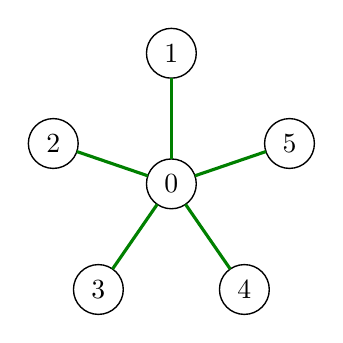
\begin{tikzpicture}
\definecolor{cv0}{rgb}{0.0,0.0,0.0}
\definecolor{cfv0}{rgb}{1.0,1.0,1.0}
\definecolor{clv0}{rgb}{0.0,0.0,0.0}
\definecolor{cv1}{rgb}{0.0,0.0,0.0}
\definecolor{cfv1}{rgb}{1.0,1.0,1.0}
\definecolor{clv1}{rgb}{0.0,0.0,0.0}
\definecolor{cv2}{rgb}{0.0,0.0,0.0}
\definecolor{cfv2}{rgb}{1.0,1.0,1.0}
\definecolor{clv2}{rgb}{0.0,0.0,0.0}
\definecolor{cv3}{rgb}{0.0,0.0,0.0}
\definecolor{cfv3}{rgb}{1.0,1.0,1.0}
\definecolor{clv3}{rgb}{0.0,0.0,0.0}
\definecolor{cv4}{rgb}{0.0,0.0,0.0}
\definecolor{cfv4}{rgb}{1.0,1.0,1.0}
\definecolor{clv4}{rgb}{0.0,0.0,0.0}
\definecolor{cv5}{rgb}{0.0,0.0,0.0}
\definecolor{cfv5}{rgb}{1.0,1.0,1.0}
\definecolor{clv5}{rgb}{0.0,0.0,0.0}
\definecolor{cv0v1}{rgb}{0.0,0.502,0.0}
\definecolor{cv0v2}{rgb}{0.0,0.502,0.0}
\definecolor{cv0v3}{rgb}{0.0,0.502,0.0}
\definecolor{cv0v4}{rgb}{0.0,0.502,0.0}
\definecolor{cv0v5}{rgb}{0.0,0.502,0.0}
%
\Vertex[style={minimum size=0.2cm,draw=cv0,fill=cfv0,text=clv0,shape=circle},LabelOut=false,L=\hbox{$0$},x=1.5cm,y=1.3416cm]{v0}
\Vertex[style={minimum size=0.2cm,draw=cv1,fill=cfv1,text=clv1,shape=circle},LabelOut=false,L=\hbox{$1$},x=1.5cm,y=3.0cm]{v1}
\Vertex[style={minimum size=0.2cm,draw=cv2,fill=cfv2,text=clv2,shape=circle},LabelOut=false,L=\hbox{$2$},x=0.0cm,y=1.8541cm]{v2}
\Vertex[style={minimum size=0.2cm,draw=cv3,fill=cfv3,text=clv3,shape=circle},LabelOut=false,L=\hbox{$3$},x=0.5729cm,y=0.0cm]{v3}
\Vertex[style={minimum size=0.2cm,draw=cv4,fill=cfv4,text=clv4,shape=circle},LabelOut=false,L=\hbox{$4$},x=2.4271cm,y=0.0cm]{v4}
\Vertex[style={minimum size=0.2cm,draw=cv5,fill=cfv5,text=clv5,shape=circle},LabelOut=false,L=\hbox{$5$},x=3.0cm,y=1.8541cm]{v5}
%
\Edge[lw=0.04cm,style={color=cv0v1,},](v0)(v1)
\Edge[lw=0.04cm,style={color=cv0v2,},](v0)(v2)
\Edge[lw=0.04cm,style={color=cv0v3,},](v0)(v3)
\Edge[lw=0.04cm,style={color=cv0v4,},](v0)(v4)
\Edge[lw=0.04cm,style={color=cv0v5,},](v0)(v5)
%
\end{tikzpicture}
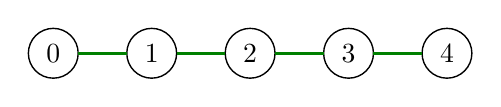
\begin{tikzpicture}
\definecolor{cv0}{rgb}{0.0,0.0,0.0}
\definecolor{cfv0}{rgb}{1.0,1.0,1.0}
\definecolor{clv0}{rgb}{0.0,0.0,0.0}
\definecolor{cv1}{rgb}{0.0,0.0,0.0}
\definecolor{cfv1}{rgb}{1.0,1.0,1.0}
\definecolor{clv1}{rgb}{0.0,0.0,0.0}
\definecolor{cv2}{rgb}{0.0,0.0,0.0}
\definecolor{cfv2}{rgb}{1.0,1.0,1.0}
\definecolor{clv2}{rgb}{0.0,0.0,0.0}
\definecolor{cv3}{rgb}{0.0,0.0,0.0}
\definecolor{cfv3}{rgb}{1.0,1.0,1.0}
\definecolor{clv3}{rgb}{0.0,0.0,0.0}
\definecolor{cv4}{rgb}{0.0,0.0,0.0}
\definecolor{cfv4}{rgb}{1.0,1.0,1.0}
\definecolor{clv4}{rgb}{0.0,0.0,0.0}
\definecolor{cv0v1}{rgb}{0.0,0.502,0.0}
\definecolor{cv1v2}{rgb}{0.0,0.502,0.0}
\definecolor{cv2v3}{rgb}{0.0,0.502,0.0}
\definecolor{cv3v4}{rgb}{0.0,0.502,0.0}
%
\Vertex[style={minimum size=0.2cm,draw=cv0,fill=cfv0,text=clv0,shape=circle},LabelOut=false,L=\hbox{$0$},x=0.0cm,y=1.5cm]{v0}
\Vertex[style={minimum size=0.2cm,draw=cv1,fill=cfv1,text=clv1,shape=circle},LabelOut=false,L=\hbox{$1$},x=1.25cm,y=1.5cm]{v1}
\Vertex[style={minimum size=0.2cm,draw=cv2,fill=cfv2,text=clv2,shape=circle},LabelOut=false,L=\hbox{$2$},x=2.5cm,y=1.5cm]{v2}
\Vertex[style={minimum size=0.2cm,draw=cv3,fill=cfv3,text=clv3,shape=circle},LabelOut=false,L=\hbox{$3$},x=3.75cm,y=1.5cm]{v3}
\Vertex[style={minimum size=0.2cm,draw=cv4,fill=cfv4,text=clv4,shape=circle},LabelOut=false,L=\hbox{$4$},x=5.0cm,y=1.5cm]{v4}
%
\Edge[lw=0.04cm,style={color=cv0v1,},](v0)(v1)
\Edge[lw=0.04cm,style={color=cv1v2,},](v1)(v2)
\Edge[lw=0.04cm,style={color=cv2v3,},](v2)(v3)
\Edge[lw=0.04cm,style={color=cv3v4,},](v3)(v4)
%
\end{tikzpicture}
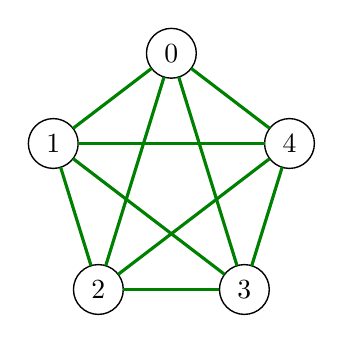
\begin{tikzpicture}
\definecolor{cv0}{rgb}{0.0,0.0,0.0}
\definecolor{cfv0}{rgb}{1.0,1.0,1.0}
\definecolor{clv0}{rgb}{0.0,0.0,0.0}
\definecolor{cv1}{rgb}{0.0,0.0,0.0}
\definecolor{cfv1}{rgb}{1.0,1.0,1.0}
\definecolor{clv1}{rgb}{0.0,0.0,0.0}
\definecolor{cv2}{rgb}{0.0,0.0,0.0}
\definecolor{cfv2}{rgb}{1.0,1.0,1.0}
\definecolor{clv2}{rgb}{0.0,0.0,0.0}
\definecolor{cv3}{rgb}{0.0,0.0,0.0}
\definecolor{cfv3}{rgb}{1.0,1.0,1.0}
\definecolor{clv3}{rgb}{0.0,0.0,0.0}
\definecolor{cv4}{rgb}{0.0,0.0,0.0}
\definecolor{cfv4}{rgb}{1.0,1.0,1.0}
\definecolor{clv4}{rgb}{0.0,0.0,0.0}
\definecolor{cv0v1}{rgb}{0.0,0.502,0.0}
\definecolor{cv0v2}{rgb}{0.0,0.502,0.0}
\definecolor{cv0v3}{rgb}{0.0,0.502,0.0}
\definecolor{cv0v4}{rgb}{0.0,0.502,0.0}
\definecolor{cv1v2}{rgb}{0.0,0.502,0.0}
\definecolor{cv1v3}{rgb}{0.0,0.502,0.0}
\definecolor{cv1v4}{rgb}{0.0,0.502,0.0}
\definecolor{cv2v3}{rgb}{0.0,0.502,0.0}
\definecolor{cv2v4}{rgb}{0.0,0.502,0.0}
\definecolor{cv3v4}{rgb}{0.0,0.502,0.0}
%
\Vertex[style={minimum size=0.2cm,draw=cv0,fill=cfv0,text=clv0,shape=circle},LabelOut=false,L=\hbox{$0$},x=1.5cm,y=3.0cm]{v0}
\Vertex[style={minimum size=0.2cm,draw=cv1,fill=cfv1,text=clv1,shape=circle},LabelOut=false,L=\hbox{$1$},x=0.0cm,y=1.8541cm]{v1}
\Vertex[style={minimum size=0.2cm,draw=cv2,fill=cfv2,text=clv2,shape=circle},LabelOut=false,L=\hbox{$2$},x=0.5729cm,y=0.0cm]{v2}
\Vertex[style={minimum size=0.2cm,draw=cv3,fill=cfv3,text=clv3,shape=circle},LabelOut=false,L=\hbox{$3$},x=2.4271cm,y=0.0cm]{v3}
\Vertex[style={minimum size=0.2cm,draw=cv4,fill=cfv4,text=clv4,shape=circle},LabelOut=false,L=\hbox{$4$},x=3.0cm,y=1.8541cm]{v4}
%
\Edge[lw=0.04cm,style={color=cv0v1,},](v0)(v1)
\Edge[lw=0.04cm,style={color=cv0v2,},](v0)(v2)
\Edge[lw=0.04cm,style={color=cv0v3,},](v0)(v3)
\Edge[lw=0.04cm,style={color=cv0v4,},](v0)(v4)
\Edge[lw=0.04cm,style={color=cv1v2,},](v1)(v2)
\Edge[lw=0.04cm,style={color=cv1v3,},](v1)(v3)
\Edge[lw=0.04cm,style={color=cv1v4,},](v1)(v4)
\Edge[lw=0.04cm,style={color=cv2v3,},](v2)(v3)
\Edge[lw=0.04cm,style={color=cv2v4,},](v2)(v4)
\Edge[lw=0.04cm,style={color=cv3v4,},](v3)(v4)
%
\end{tikzpicture}



    \centering
    \caption{Star, path and complete networks with $n=5$. Lines should be interpreted as a bidirectional connection.}
    \label{threetrees}
\end{figure}

In Section \ref{si-model-section}, we only briefly mentioned the transmission tree, but in this section, we take a closer look at its construction and what it entails. The transmission tree describes the path of the contagion as it traverses between the nodes. The tree is a leaf-labelled ranked planar binary tree with the leaf-labels being node labels, where the left leaf is the infector and the right leaf the infectee. As an infected node spread the infection to a susceptible neighbour, the leaf will be transformed into an sub-terminal vertex labelled with an integer describing the infection number. Figure \ref{treeexample} shows an example of how the tree is built. $n_0$ is the initially infected node. The first infection was spread from $n_0$ to $n_2$. The second was from $n_2$ to $n_4$. Third infection from $n_2$ to $n_3$, and fourth $n_4$ to $n_1$. Figure \ref{transexample} shows this transmission process on a complete network with $n=5$. Infected nodes are red and susceptible nodes green. Lines should be interpreted as bidirectional connections, where red lines represent infectious contacts, and green ones non-infectious. 
\begin{figure}[H]
    \centering
    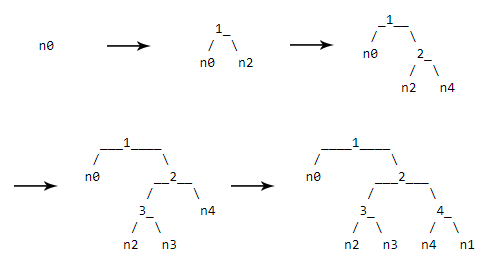
\includegraphics[scale=0.5]{treeexample.png}   
    \caption{An example of how the tree is constructed. The order of transmission is $n_0\rightarrow n_2\rightarrow n_4\rightarrow n_3\rightarrow n_1$.}
    \label{treeexample}
\end{figure}
\begin{figure}[H]
    \centering
    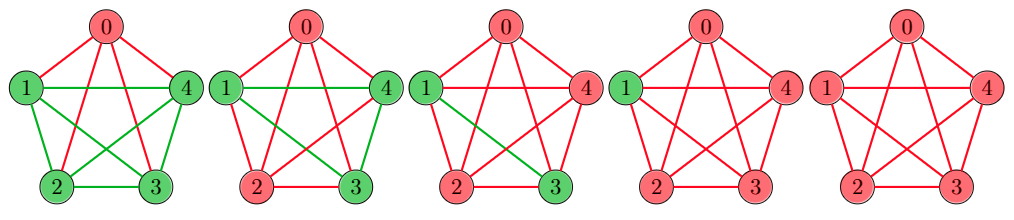
\includegraphics[scale=0.35]{exTrans.png}   
    \caption{An example of transmission on a complete network with $n=5$ using SI-model. The initial state is the leftmost pentagram. The order of transmission is $n_0\rightarrow n_2\rightarrow n_4\rightarrow n_3\rightarrow n_1$.}
    \label{transexample}
\end{figure}

The pattern to finding the infector/infectee pair of k-th infection from a transmission tree is simple; let $LT(k)$ be the left sub-tree from internal vertex labelled k, and $RT(k)$ its right sub-tree. $LT(k)$ and $RT(k)$ might be a tree or simply a leaf label. Then, the infector of the k-th infection is the leaf label located furthest to the left of $LT(k)$ and the infectee is the node furthest to the left of $RT(k)$. For figure \ref{bigtree}, if we wish to find the infector/infectee pair of infection number 6, then we begin by finding the sub-terminal vertex labelled 6. Then, find the leftmost leaf in the left tree, which is in this case $n_2$, and thus is our infector. The infectee is the leftmost leaf in the right tree, which is $n_7$. Therefore, infection event number 6 is $n_2 \rightarrow n_7$.
\begin{figure}[H]
    \centering
    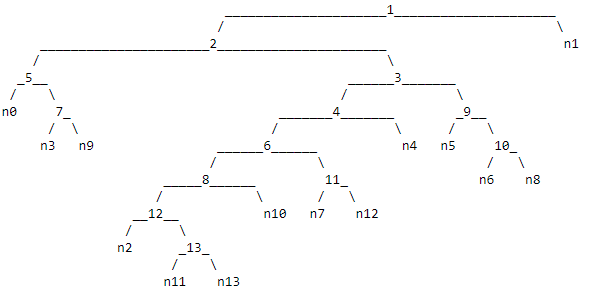
\includegraphics[scale=0.7]{bigtree.png}   
    \caption{A bigger example of a transmission tree with 13 infection events.}
    \label{bigtree}
\end{figure}


The deterministic networks in figure \ref{threetrees} are the limiting cases for the shape of the transmission tree. When using the SIR-model, a star network have only one possible infector, namely the star node. Therefore, any infection will always be spread from the star node, so the tree always splits to the left. The structure of the tree will then be shaped down to the left. It is the opposite for the path network; the newest infectee with always be the next infector, and so the tree is shaped to the right. Figure \ref{pathstartree} shows this behaviour. The complete network is a different deal, any shape of the tree have an equal probability of occurring since there is no bias toward any node in any way. Figure \ref{bigtree} can be a realization of transmission on a complete network.
\begin{figure}
    \centering
    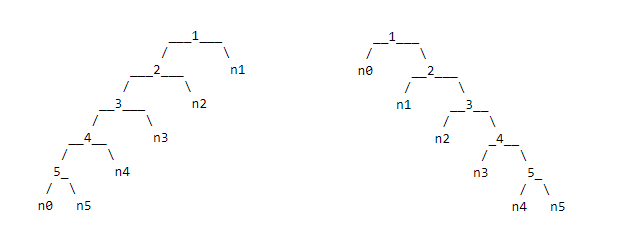
\includegraphics[scale=0.7]{starpathtree.png}   
    \caption{The shape of the transmission tree when the network is star (left) or path (right).}
    \label{pathstartree}
\end{figure}
\FloatBarrier


\section{Simulating transmission on networks}\label{simulation-section}
In this section, we simulate transmission on different networks using SIR-, and SIS-models and present the result. The simulator is written in sagemath using python 3.x, the code is openly available at \cite{github}. Simulations are run using commands $$SIR(C,\lambda_1,\lambda_2),$$ $$SIS(C,\lambda_1,\lambda_2,z_{end})$$
for SIR-, and SIS-models, respectively. $z_{end}$ is the maximum allowed events before simulation end. Parameters $\lambda_{1}$ and $\lambda_{2}$ are the rates at which state changes happen; $\lambda_1$ is the rate at which a susceptible node turns infected per infected neighbour $S\rightarrow I$, i.e. the and n is the number of nodes ($n=30$ for all simulations). $\lambda_2$ depends on the model, it's the rate of $I\rightarrow R$ for the SIR-model, or the rate of $I\rightarrow S$ for the SIS-model. C is an arbitrary bidirectional network. The three deterministic networks are created with command $$C = graphs.StarGraph(n).to\_directed(),$$ $$C = graphs.PathGraph(n).to\_directed(),$$ $$C = graphs.CompleteGraph(n).to\_directed().$$

The simulator does the following for every event; 
\begin{itemize}
    \item generate the transition probabilities from equation \ref{SIR-P12}. This equation is also valid for the SIS-model.
    \item generate a random variable p, uniformly distributed between 0 and 1. If $p<\delta_z$, then step z+1 is an infection event, otherwise it is a recovery event.
    \item if the next step is an infection event, choose a uniformly random \textit{connection} and mark the susceptible node infected. On the other hand, if the next event is a recovery event, choose a random \textit{infected node} and mark it recovered (or susceptible for the SIS-model).
    \item stop simulation if there are no more infected nodes or if $z_{end}$ events have occurred.
\end{itemize}

Since we're choosing a random \textit{connection} in the case of an infection event, susceptible nodes with more infected neighbours are more likely to become infected. Nodes with twice as many infected neighbours have a twice as high probability of being selected. $\lambda_1$ will be set to 1, while $\lambda_2$ varies between models and simulations. 

The result of the simulations will be analysed differently depending on the type of model. The goal of simulations using the SIR-model is to study the frequency of simulations ending with a certain count of recovered nodes (as opposed to still susceptible). The SIS-model have a different statistic that is more interesting to study; the frequency of each individual node being an infector or infectee.



\subsection{Simulations using SIR-model}\label{SIRsimsection}
There is a probability that the infection only affects a subset of the nodes before we get enough recovery events for the infection to die out, not all simulations will end with every node being recovered. Simulations will always end with every node being either recovered or susceptible. This section's point of interest is looking at how many of the n nodes are recovered after the infection is gone.

We perform simulations for three different networks C (star, path, complete) with n nodes with the goal of investigating how the parameter $\lambda_2$ affect the probability of $1\leq k\leq n$ nodes being recovered after the infection is gone. Higher values of $\lambda_2$, compared to $\lambda_1$, increases the probability of recovery events and reduces the chances of nodes being untouched by the virus. 

We can find the probability of having only a single recovered node as the simulation end analytically, by simply calculating $1-\delta_0$ from equation \ref{SIR-P12}:
\begin{equation}\label{bara1}
    P(\text{1 recovered}) = 1-\delta_0 = \frac{\lambda_2}{n_0^{(c)}\lambda_1+\lambda_2}.
\end{equation}
We calculate the expected frequency for ending a simulation with 1 or 2 recovered nodes and compare it to the observed frequency for each network and value of $\lambda_2$.

\subsubsection{Transmission on star network}\label{simsirstarsec}
These are the results of simulations ran on a star network with $n=30$. The value used for $\lambda_2$ are $1/2$, 1, 5 and 10. 1000 simulations are run for each value of of $\lambda_2$, and we look at how many nodes are recovered when simulation ends. For a star network with n = 30 and $\lambda_1 = 1$, the probability of a simulation ending with one or two recovered nodes is
\begin{equation}\label{bara1star}
    P(\text{1 recovered}) = \frac{\lambda_2}{30+\lambda_2}.
\end{equation}
\begin{align}\label{bara2star}
    P(\text{2 recovered}) = \delta_0\Big(\frac{1-\delta_1}{2}+\frac{1-\delta_1}{2}(1-\delta_2)\Big) = & \\ \frac{30\lambda_2}{(30+\lambda_2){(29+\lambda_2)}}
\end{align}
\begin{figure}[H]
    \centering
    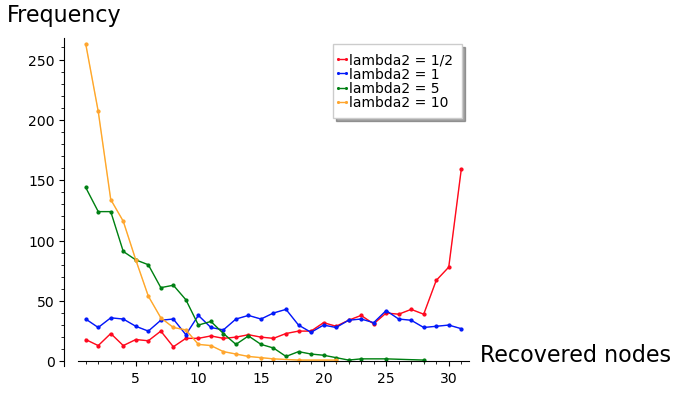
\includegraphics[scale=0.7]{starSIR.png}   
    \caption{Result of simulation of transmission on a star network for $\lambda_1 = 1$ and $\lambda_2 = 1/2,1,5,10$. 1000 simulations for each $\lambda_2$. The x-axis shows the number of recovered nodes when there are no more infected nodes. The y-axis shows how many the frequency of simulations ending with x recovered nodes.}
    \label{starsirplot}
\end{figure}
\begin{table}
    \centering
   \begin{tabular}{c|c|c|c|c}
     $\lambda_2$&  A& B& C&D\\
     1/2& 16.4& 18&16.67&13 \\
     1& 32.25&35&32.25&28 \\
     5& 142.85&144 &124&110  \\
     10& 250& 263 &192.3&207 \\
\end{tabular} 
    \label{tablestarsir}
    \caption{Expected and observed frequency of simulations ending with 1 or 2 recovered nodes. Group A is expected frequency of 1 recovered node and group B is its observed frequency. Group C is expected frequency of 2 recovered nodes and group D is its observed frequency.}
\end{table}
The red data represent the simulations when $\lambda_2 = 1/2$. All frequencies are greater than 0. The vast majority (over 150) ended with with all nodes being recovered, meaning the virus affected every node in the system. The theoretical value for how many simulations out of 1000 that ended with only 1 recovered node using $\lambda_2 = 1/2$ (equation \ref{bara1}) is 16.4 and we observed 18. The theoretical value for 2 recovered nodes is 16.67, and we observed 13. 

Blue data represent $\lambda_2 = 1$ and is almost completely uniform. The expected number of simulations ending with either 1 or 2 recovered nodes are equal for the star network using $\lambda_2 = 1$ is equal to 32.25. We observed 35 simulations ending with 1 recovered node and 28 ending with 2 recovered nodes.

The green data represent $\lambda_2=5$, and had no simulations end with more than 27 recovered nodes. Since $\lambda_2$ is much larger than before, we see more simulations end with fewer recovered nodes, because the probability of a recovery event has been greatly increased. The expected number of simulations ending with 1 recovered node is 142.85 and we observed 144. The expected number of simulations ending with 2 recovered node is 124 and we observed 110.


The yellow data are for $\lambda_2 = 10$. When $\lambda_2 = 10$, the expected number of simulations ending with 1 recovered node is 250 and we observed 263. The expected number of simulations ending with 2 recovered node is 192.3 and we observed 207.

\subsubsection{Transmission on path network}
This is the result of simulations run on a path network with $n=30$. The value used for $\lambda_2$ are $1/16$, $1/8$, $1/3$, and 1. 1000 simulations are run for each value of $\lambda_2$, and we look at the number of unaffected susceptible nodes, as we did before. An important aspect of the path network is the fact that there is always only one infectious connection at any given time. There might be several infected nodes, but only a single susceptible node can have an infected neighbour. If the rightmost infected node recovers, then the contagion is limited to the nodes to the left of it, and the outbreak is effectively over. For a path network with n = 30 and $\lambda_1 = 1$, the probability of a simulation ending with one or two recovered nodes is
\begin{equation}\label{bara1path}
    P(\text{1 recovered}) = \frac{\lambda_2}{1+\lambda_2}.
\end{equation}
\begin{align}\label{bara2path}
    P(\text{2 recovered}) = \delta_0\Big(\frac{1-\delta_1}{2}+\frac{1-\delta_1}{2}(1-\delta_2)\Big) = & \\ \frac{\lambda_2}{(1+\lambda_2)(1+\lambda_2)}
\end{align}
\begin{figure}
    \centering
    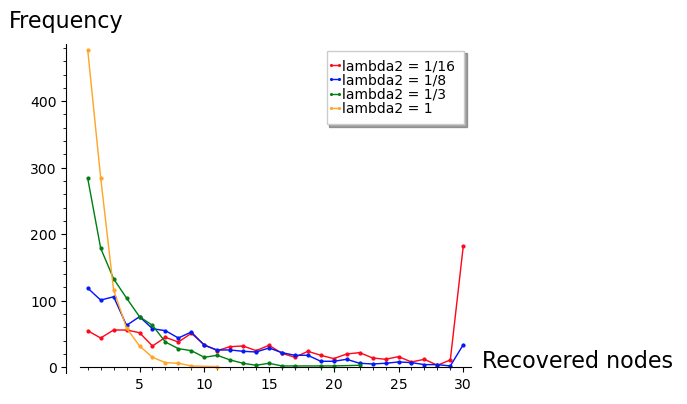
\includegraphics[scale=0.7]{pathSIR.png}   
    \caption{Result of 1000 simulations of transmission on a path network for $\lambda_1 = 1$ and $\lambda_2 = 1/16, 1/8, 1/3, 1$. The x-axis shows the number of recovered nodes when there are no more infected nodes. The y-axis shows how many the frequency of simulations ending with x recovered nodes.}
    \label{pathsirplot}
\end{figure}

\begin{table}
    \centering
   \begin{tabular}{c|c|c|c|c}
     $\lambda_2$&  A& B& C&D\\
     1& 500& 477 &250&285 \\
     1/3& 250& 284 &187.5&179 \\
     1/8& 111.1& 119 &98.8&101  \\
     1/16& 58.8& 55 &55.4&44\\
\end{tabular} 
    \label{tablepathsir}
    \caption{Expected and observed frequency of simulations ending with 1 or 2 recovered nodes. Group A is expected frequency of 1 recovered node and group B is its observed frequency. Group C is expected frequency of 2 recovered nodes and group D is its observed frequency.}
\end{table}

Looking at figure \ref{pathsirplot}, we generally see that for higher values of $\lambda_2$, fewer nodes are recovered when the virus is gone. The yellow dots represent $\lambda_2 = 1$ and most simulations with this value end without infecting any other node. No simulations ended with more than 11 recovered nodes. $\lambda_2 = 1$ is the value most likely to end with one or two recovered nodes. The expected number of simulations ending with 1 recovered node is 500, and we observed 477. The equivalent statistic for 250 recovered nodes is 250 and we observed 285.

The green data is for $\lambda_2 = 1/3$. We see that it is still very likely to only infect very few nodes before the virus is gone. This value is the most likely to end with three to five recovered nodes. The expected number of simulations ending with 1 recovered node is 250, and we observed 284. The equivalent statistic for 2 recovered nodes is 187.5 and we observed 179.

The blue data is for $\lambda_2 = 1/8$. We see for the first time counts for 0 susceptible nodes, although they are quite a few. This value for $\lambda_2$ is the most likely to end with around 6-11 recovered nodes. The expected number of simulations ending with 1 recovered node is 111.1, and we observed 119. The equivalent statistic for 2 recovered nodes is 98.8 and we observed 101.

Lastly, we have the red data for $\lambda_2 = 1/16$. There is a spike at 30 recovered nodes, because infection events are very likely until every node have been infected. This value is the most likely to end with 0-16 nodes. The expected number of simulations ending with 1 recovered node is 58.8, and we observed 55. The equivalent statistic for 2 recovered nodes is 55.4 and we observed 44.
\FloatBarrier
\subsubsection{Transmission on complete network}\label{simsircomsec}
This is the result of simulations ran on a complete network with $n=30$. The value used for $\lambda_2$ are $5$, $10$, $15$, $20$, and $25$. 1000 simulations are run for each value of of $\lambda_2$. For a complete network with n = 30 and $\lambda_1 = 1$, the probability of a simulation ending with one or two recovered nodes is
\begin{equation}\label{bara1complete}
    P(\text{1 recovered}) = \frac{\lambda_2}{29+\lambda_2}.
\end{equation}
\begin{align}\label{bara2complete}
    P(\text{2 recovered}) = 2\delta_0(1-\delta_1)(1-\delta_2) = & \\ \frac{29\lambda_2^2}{(29+\lambda_2)(28+\lambda_2)^2}.
\end{align}
\begin{figure}[H]
    \centering
    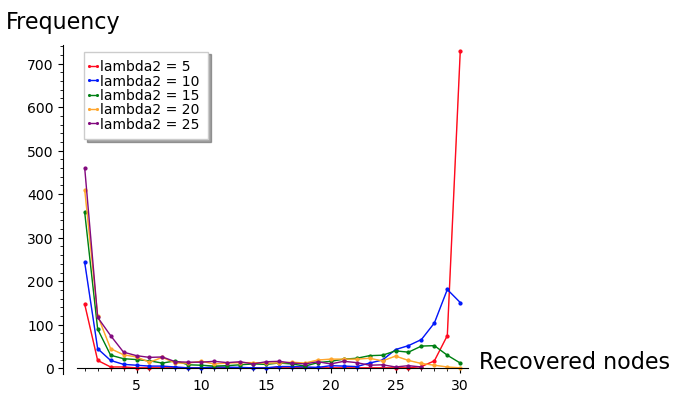
\includegraphics[scale=0.7]{completeSIR.png}   
    \caption{Result of 1000 simulations of transmission on a complete network for $\lambda_2 = 5,10,15,20,25$. The x-axis shows the number of susceptible nodes left unaffected by the virus when simulation ended. y-axis shows how many simulations ended with x susceptible nodes.}
    \label{completesirplot}
\end{figure}
\begin{table}[H]
    \centering
   \begin{tabular}{c|c|c|c|c}
     $\lambda_2$&  A& B& C&D\\
     5& 147& 147 &19.6&18 \\
     10& 256.4& 243 &51.5&45 \\
     15& 340.9& 358&80.2&90  \\
     20& 408.2& 410 &102.7&121\\
     25& 463& 460 &119.5&117\\
\end{tabular} 
    \label{tablecompletesir}
    \caption{Expected and observed frequency of simulations ending with 1 or 2 recovered nodes. Group A is expected frequency of 1 recovered node and group B is its observed frequency. Group C is expected frequency of 2 recovered nodes and group D is its observed frequency.}
\end{table}
The vast majority of simulations with $\lambda_2 = 5$ ended with all nodes being infected, only very few ended with 1 or 2 nodes. As $\lambda_2$ grows, there are fewer and fewer counts of 30 recovered nodes, but the frequency for fewer recovered nodes increases. The expected number of simulations ending with 1 recovered node is 147, and we observed exactly 147. The equivalent statistic for 2 recovered nodes is 19.6 and we observed 18.

The blue data represents $\lambda_2=10$, which has a greater frequency of only 1 or 2 recovered nodes than $\lambda_2 = 5$. This line has a "bump" at 29, which can be seen "moving" left-ward as $\lambda_2$ grows. The expected number of simulations ending with 1 recovered node is 256.4, and we observed 243. The equivalent statistic for 2 recovered nodes is 51.5 and we observed 45.

The green data represents $\lambda_2 = 15$ and we see that the trend continues as the frequency for fewer recovered nodes increases but is almost zero for 30. The bump has moved a bit to the left and is now not as high. The expected number of simulations ending with 1 recovered node is 340.9, and we observed 258. The equivalent statistic for 2 recovered nodes is 80.2 and we observed 90.

The yellow data represents $\lambda_2 = 20$. The bump is not as prominent as before but there is a rise in frequencies around 25 recovered nodes. The expected number of simulations ending with 1 recovered node is 408.2, and we observed exactly 410. The equivalent statistic for 2 recovered nodes is 102.7 and we observed 121.

The green data represents $\lambda_2 = 25$. The expected number of simulations ending with 1 recovered node is 463, and we observed exactly 460. The equivalent statistic for 2 recovered nodes is 119.5 and we observed 117.




\subsection{Simulations using SIS-model}\label{SISsimsection}
In this section, we perform simulations for four different networks C (= star, path, complete and small world). There is no point in running several simulations since the point of interest here is the long-term behaviour of the equilibrium, and not necessarily the final outcome. We begin by introducing a new notation, let $f^1_i$ be the frequency of node i being an infector and $f^2_i$ be the frequency of node i being an infectee. Let $\Bar{f}^1$ and $\Bar{f}^2$ be the average of $f^1_i$ and $f^2_i$, respectively, for all relevant nodes (all nodes are considered relevant unless otherwise stated in the simulation). In these simulations, we shall be looking at the frequency of a node being an infector or infectee, i.e. $f^1_i$ and $f^2_i$, for all i. The values for $\lambda_1$ and $\lambda_2$ are mostly trivial, only changed to ensure the infection isn't gone before $z_{end}$ events have occurred.

\subsubsection{Transmission of star network}\label{simsis1}
For the star network with n outer nodes, we expect all outer nodes to have approximately equal infector/infectee frequencies. The infectee frequency for the star node is the sum of the frequency of outer nodes being the infector. Similarly, the star node's infector frequency is the sum of the outer nodes' infectee frequencies. Let $\lambda_1 = 3$, $\lambda_2 = 1$ and $z_{end} = 5000$.

\begin{figure}
    \centering
    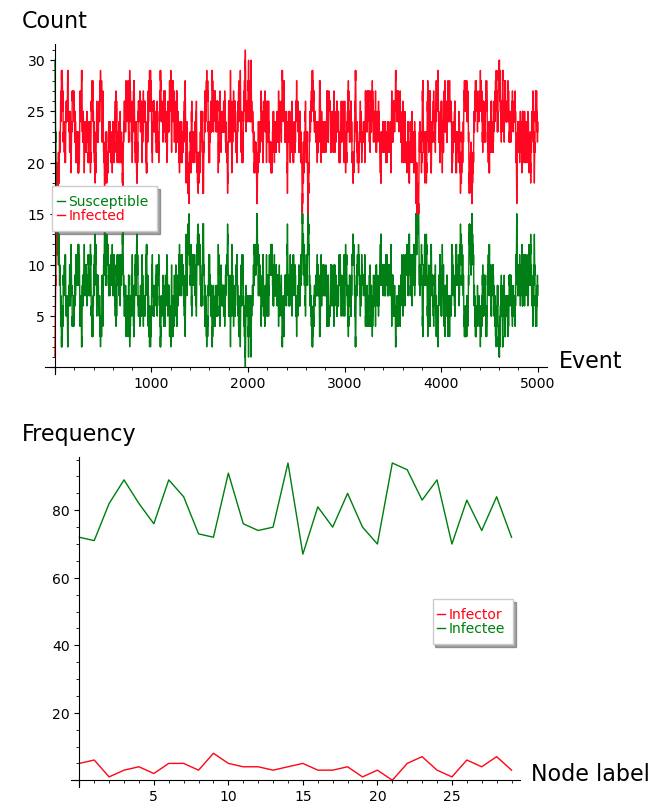
\includegraphics[scale=0.7]{SISstar1.png}   
    \caption{The top figure shows number of infected and susceptible nodes after step z for a star network with $n = 30$ using an SIS-model. Bottom figure shows the infector/infectee frequencies for all nodes, except the star node.}
    \label{starSISplot1}
\end{figure}
The top of figure \ref{starSISplot1} shows the number of infected (red) and susceptible (green) nodes after each step. The simulation reveals the oscillating behaviour of the SIS-model with the red and green graphs going back and forth with different amplitudes each time. Smaller amplitudes are more likely to occur than larger amplitudes since each infection event will increase the probability of recovery events. 
\begin{table}[H]
    \centering
\begin{tabular}{c c}
     $\Bar{n}^{(s)}$ &7.76(2.67) \\ \hline 
     $\Bar{n}^{(i)}$ &23.24(2.67) \\ \hline
     $\Bar{f}^1$& 3.90(1.89) \\ \hline
     $\Bar{f}^2$&  79.8(8) \\ \hline
     $f^1_*$&  2394 \\ \hline
     $f^2_*$&  118
\end{tabular}
    \caption{Result of one 5000-event simulation of transmission on a star network using the SIS-model. The numbers in parenthesis are the sample standard deviation.}
    \label{table:sisstar}
\end{table}
The star node $n_*$ is excluded from the calculation of $\Bar{n}^{(s)}$ and $\Bar{n}^{(i)}$ since the interesting part of these statistics lies in the outer nodes.
The number of susceptible nodes oscillates around a mean value 15.13 and the infected nodes around 7.76 (which is 30-23.24, the total number of nodes minus the number of susceptible nodes). The star node is the only one with more than one connection and is expected to be an infector/infectee more often than the outer nodes, and so is excluded from the mean values $\Bar{n}^{(s)}, \Bar{n}^{(i)}$. The average number of infections caused is of course the number of times the star node have been infected times 30, the number of outer nodes. Similarly, the average number of times an outer node have been infected is 30 times infections caused by star node.
\FloatBarrier
\subsubsection{Transmission on path network}
In the path network for $n=30$ nodes, we expect the nodes $n_0$ and $n_n$ to have a bit less than half of the average number of times infected. 
The simulation will be run for 15000 events. The infection rate is set to 3, while the recovery rate is set to 1. It is very unlikely to have a successful 15000-event simulation if the infection rate is too low compared to the recovery rate, since the infection is cured too fast, and therefore $\lambda_1=3$ and $\lambda_2 = 1$. 
\begin{figure}[ht]
    \centering
    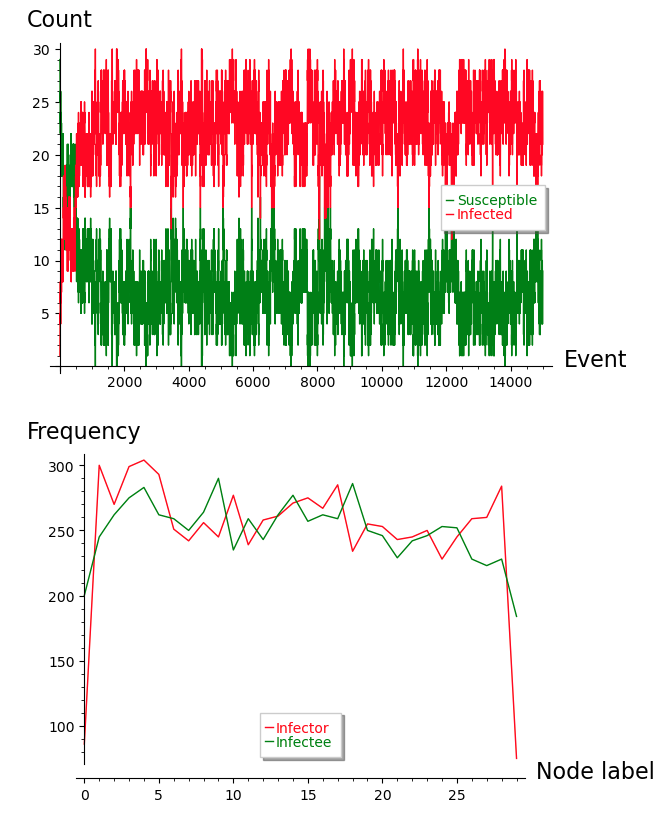
\includegraphics[scale=0.7]{SISpath1.png}   
    \caption{The top figure shows number of infected and susceptible nodes after event z for a path network with $n = 30$ using an SIS-model. Bottom figure shows the infector/infectee frequencies for all nodes.}
    \label{pathSISplot1}
\end{figure}
\begin{table}[H]
    \centering
\begin{tabular}{c|c}
     $\Bar{n}^{(s)}$ &7.34(3.4) \\ \hline 
     $\Bar{n}^{(i)}$ &22.67(3.4) \\ \hline
     $\Bar{f}^1$& 250.3(50.36)\\ \hline
     $\Bar{f}^2$&  250.36(23.34) 
\end{tabular}
    \caption{Result of one 15000-event simulation of transmission on a path network using the SIS-model. The numbers in parenthesis are the sample standard deviation.}
    \label{table:sispath}
\end{table}

The top plot of figure \ref{pathSISplot1} shows the number of susceptible and infected nodes. It inhibits the oscillating behaviour expected from an SIS-model and also seem to oscillate around some mean point, as shown in table \ref{table:sispath}. The bottom plot of figure \ref{pathSISplot1} shows the distribution of the infector/infectee frequency for all 30 nodes. The plot looks mostly uniform, but looking at $f^1_0$, $f^2_0$, $f_{29}^1$ and $f_{29}^2$, it is obvious the edge nodes (0 and 29) have a clear advantage since they only have one neighbour, whereas all other nodes have two.
\FloatBarrier
\subsubsection{Transmission on complete network}\label{simsis3}
The symmetry of the network causes all nodes to have approximately the same number of infections caused and times infected with no bias toward any node. The infection rate is set to 1, while the recovery rate is set to 5. Here, the recovery rate is higher because the probability of having a recovery event is overwhelmed by the probability of an infection event, because of the vast amount of infectious connections. If the two rates are approximately the same, the system will almost always be completely infected. The simulation will be run for 15000 events. 

\begin{figure}[ht]
    \centering
    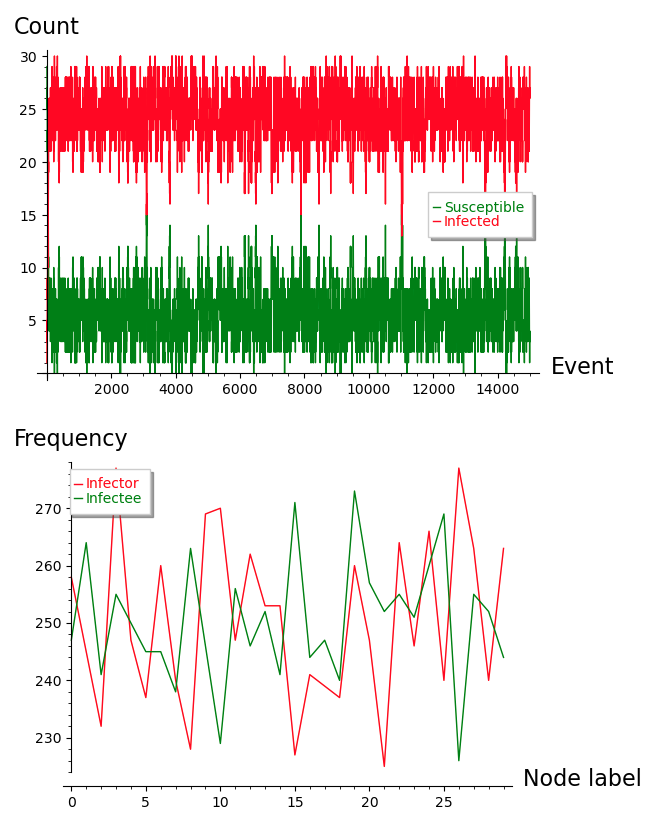
\includegraphics[scale=0.7]{SIScomplete1.png}   
    \caption{The top figure shows number of infected and susceptible nodes after step z for a complete network with $n = 30$ using an SIS-model. Bottom figure shows the infector/infectee frequencies for all nodes}
    \label{completeSISplot1}
\end{figure}
\begin{table}[H]
    \centering
\begin{tabular}{c|c}
     $\Bar{n}^{(s)}$ &5.7(2.45) \\ \hline 
     $\Bar{n}^{(i)}$ &24.3(2.45)\\ \hline
     $\Bar{f}^1$ & 250.43(14.74) \\ \hline
     $\Bar{f}^2$ & 250.46(11.08) \\ 
\end{tabular}
    \caption{Result of one 15000-event simulation of transmission on a complete network using the SIS-model. The numbers in parenthesis are the sample standard deviation.}
    \label{table:siscomplete}
\end{table}
The top plot of figure \ref{completeSISplot1} shows the oscillations happen around some equilibrium, as seen in table \ref{table:siscomplete}. The lowest amount of infected nodes seem to be around 15. When the recovery rate is five times higher than the infection rate, it seems very unlikely for the virus to be eradicated within reasonable amount of time.

The bottom plot of figure \ref{completeSISplot1} shows the distribution of $f_i^{(1)}$ and $f_i^{(2)}$ for all nodes. We see the numbers look approximately the same for all nodes with node 10 and 14 being outliers for infections caused. There seem to be no upward or downward trend in either statistic so they stay relatively constant.

\FloatBarrier
\subsubsection{Transmission on small world network}\label{smallsection}
So far we have only looked at deterministic networks where all nodes and their connections are well known before their construction. In this section, we look at a randomly generated network called the small--world network. The small-world network (also called the Newman-Watts-Strogatz network) takes three parameters as input; n, k and p. The network is constructed by first constructing a ring of n nodes, each connected to k of its nearby nodes. For each existing connection, add a new connection to a randomly chosen node with probability p. Each node will then have an expected $k(1+p)$ connections. Figure \ref{smallworldexample} shows a realisation of the small world, where the lines should be interpreted as a bidirectional connection. The topology of the network does not change after construction is complete, it is static in time. The purpose of a simulation on this network is to see the relationship between a node's infector/infectee frequency and its number of connections. 

In the case of an infection event, the infection is selected uniformly from possible infectious connections, which implies a node with more connections is more likely to be an infector/infectee than one with fewer connections. Therefore, we expect nodes with more connections will generally have a higher infector/infectee frequency. However, a node needs to recover before it can increase its infectee frequency, and the node selection in the case of a recovery event is uniform and independent of its number of neighbours. Therefore, we expect the infectee frequency to increase with its number of neighbours, but with a lower slope than the slope of the infector frequency, because of the recovery events' independence of the number of neighbours.


A 15000-event simulation is called with $$SIS(C,1,6,15000),$$ where C is a small world graph generated from $$C = graphs.RandomNewmanWattsStrogatz(300,30,0.4).to\_directed().$$ We choose not to look at $\Bar{f}^1$ and $\Bar{f}^2$ for this simulation as we did in Section \ref{simsis1}-\ref{simsis3}, since we don't have any information regarding the connections before randomization. Instead, we look at the distribution of infector/infectee frequency as a function of how many neighbours a node has, together with its average.
Figure \ref{SWresultplot} shows the result of the simulation. The top plot shows the infector frequency for each node as a function of the number of neighbours the node have. Each blue dot represents one node. The red line is the average infector frequency for a certain number of neighbours. The is an upward trend that stems from the positive relationship between the number of neighbours and its probability of infecting another node.

The bottom plot shows infectee frequency as a function of the number of neighbours a node has. As expected, the trend is mostly uniform, but with a slight upward, although not as prominent as it is for the top plot. 

We conclude there is a positive correlation between the infector/infectee frequency and the number of neighbours.


\begin{figure}[H]
    \centering
    
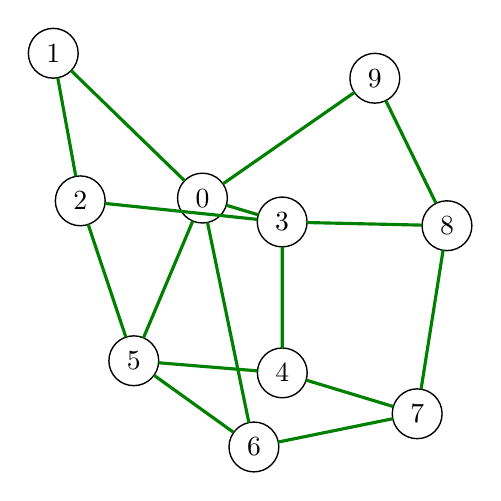
\begin{tikzpicture}
\definecolor{cv0}{rgb}{0.0,0.502,0.0}
\definecolor{cfv0}{rgb}{1.0,1.0,1.0}
\definecolor{clv0}{rgb}{1.0,0.0,0.0}
\definecolor{cv1}{rgb}{0.0,0.502,0.0}
\definecolor{cfv1}{rgb}{1.0,1.0,1.0}
\definecolor{clv1}{rgb}{1.0,0.0,0.0}
\definecolor{cv2}{rgb}{0.0,0.502,0.0}
\definecolor{cfv2}{rgb}{1.0,1.0,1.0}
\definecolor{clv2}{rgb}{1.0,0.0,0.0}
\definecolor{cv3}{rgb}{0.0,0.502,0.0}
\definecolor{cfv3}{rgb}{1.0,1.0,1.0}
\definecolor{clv3}{rgb}{1.0,0.0,0.0}
\definecolor{cv4}{rgb}{0.0,0.502,0.0}
\definecolor{cfv4}{rgb}{1.0,1.0,1.0}
\definecolor{clv4}{rgb}{1.0,0.0,0.0}
\definecolor{cv5}{rgb}{0.0,0.502,0.0}
\definecolor{cfv5}{rgb}{1.0,1.0,1.0}
\definecolor{clv5}{rgb}{1.0,0.0,0.0}
\definecolor{cv6}{rgb}{0.0,0.502,0.0}
\definecolor{cfv6}{rgb}{1.0,1.0,1.0}
\definecolor{clv6}{rgb}{1.0,0.0,0.0}
\definecolor{cv7}{rgb}{0.0,0.502,0.0}
\definecolor{cfv7}{rgb}{1.0,1.0,1.0}
\definecolor{clv7}{rgb}{1.0,0.0,0.0}
\definecolor{cv8}{rgb}{0.0,0.502,0.0}
\definecolor{cfv8}{rgb}{1.0,1.0,1.0}
\definecolor{clv8}{rgb}{1.0,0.0,0.0}
\definecolor{cv9}{rgb}{0.0,0.502,0.0}
\definecolor{cfv9}{rgb}{1.0,1.0,1.0}
\definecolor{clv9}{rgb}{1.0,0.0,0.0}
\definecolor{cv0v1}{rgb}{0.0,0.502,0.0}
\definecolor{cv0v3}{rgb}{0.0,0.502,0.0}
\definecolor{cv0v5}{rgb}{0.0,0.502,0.0}
\definecolor{cv0v6}{rgb}{0.0,0.502,0.0}
\definecolor{cv0v9}{rgb}{0.0,0.502,0.0}
\definecolor{cv1v2}{rgb}{0.0,0.502,0.0}
\definecolor{cv2v3}{rgb}{0.0,0.502,0.0}
\definecolor{cv2v5}{rgb}{0.0,0.502,0.0}
\definecolor{cv3v4}{rgb}{0.0,0.502,0.0}
\definecolor{cv3v8}{rgb}{0.0,0.502,0.0}
\definecolor{cv4v5}{rgb}{0.0,0.502,0.0}
\definecolor{cv4v7}{rgb}{0.0,0.502,0.0}
\definecolor{cv5v6}{rgb}{0.0,0.502,0.0}
\definecolor{cv6v7}{rgb}{0.0,0.502,0.0}
\definecolor{cv7v8}{rgb}{0.0,0.502,0.0}
\definecolor{cv8v9}{rgb}{0.0,0.502,0.0}
%
\Vertex[style={minimum size=0.2cm,draw=cv0,fill=cfv0,text=clv0,shape=circle},LabelOut=false,L=\hbox{$0$},x=1.8947cm,y=3.1608cm]{v0}
\Vertex[style={minimum size=0.2cm,draw=cv1,fill=cfv1,text=clv1,shape=circle},LabelOut=false,L=\hbox{$1$},x=0.0cm,y=5.0cm]{v1}
\Vertex[style={minimum size=0.2cm,draw=cv2,fill=cfv2,text=clv2,shape=circle},LabelOut=false,L=\hbox{$2$},x=0.3428cm,y=3.126cm]{v2}
\Vertex[style={minimum size=0.2cm,draw=cv3,fill=cfv3,text=clv3,shape=circle},LabelOut=false,L=\hbox{$3$},x=2.9069cm,y=2.8575cm]{v3}
\Vertex[style={minimum size=0.2cm,draw=cv4,fill=cfv4,text=clv4,shape=circle},LabelOut=false,L=\hbox{$4$},x=2.9086cm,y=0.9409cm]{v4}
\Vertex[style={minimum size=0.2cm,draw=cv5,fill=cfv5,text=clv5,shape=circle},LabelOut=false,L=\hbox{$5$},x=1.0226cm,y=1.0949cm]{v5}
\Vertex[style={minimum size=0.2cm,draw=cv6,fill=cfv6,text=clv6,shape=circle},LabelOut=false,L=\hbox{$6$},x=2.5482cm,y=0.0cm]{v6}
\Vertex[style={minimum size=0.2cm,draw=cv7,fill=cfv7,text=clv7,shape=circle},LabelOut=false,L=\hbox{$7$},x=4.6215cm,y=0.4216cm]{v7}
\Vertex[style={minimum size=0.2cm,draw=cv8,fill=cfv8,text=clv8,shape=circle},LabelOut=false,L=\hbox{$8$},x=5.0cm,y=2.8101cm]{v8}
\Vertex[style={minimum size=0.2cm,draw=cv9,fill=cfv9,text=clv9,shape=circle},LabelOut=false,L=\hbox{$9$},x=4.0839cm,y=4.6829cm]{v9}
%
\Edge[lw=0.04cm,style={color=cv0v1,},](v0)(v1)
\Edge[lw=0.04cm,style={color=cv0v3,},](v0)(v3)
\Edge[lw=0.04cm,style={color=cv0v5,},](v0)(v5)
\Edge[lw=0.04cm,style={color=cv0v6,},](v0)(v6)
\Edge[lw=0.04cm,style={color=cv0v9,},](v0)(v9)
\Edge[lw=0.04cm,style={color=cv1v2,},](v1)(v2)
\Edge[lw=0.04cm,style={color=cv2v3,},](v2)(v3)
\Edge[lw=0.04cm,style={color=cv2v5,},](v2)(v5)
\Edge[lw=0.04cm,style={color=cv3v4,},](v3)(v4)
\Edge[lw=0.04cm,style={color=cv3v8,},](v3)(v8)
\Edge[lw=0.04cm,style={color=cv4v5,},](v4)(v5)
\Edge[lw=0.04cm,style={color=cv4v7,},](v4)(v7)
\Edge[lw=0.04cm,style={color=cv5v6,},](v5)(v6)
\Edge[lw=0.04cm,style={color=cv6v7,},](v6)(v7)
\Edge[lw=0.04cm,style={color=cv7v8,},](v7)(v8)
\Edge[lw=0.04cm,style={color=cv8v9,},](v8)(v9)
%
\end{tikzpicture}
\caption{An example of a small-world network with $n=10$, $k=3$, $p=0.8$. Each line should be interpreted as a bidirectional connection.}
    \label{smallworldexample}
\end{figure}

\begin{figure}
    \centering
    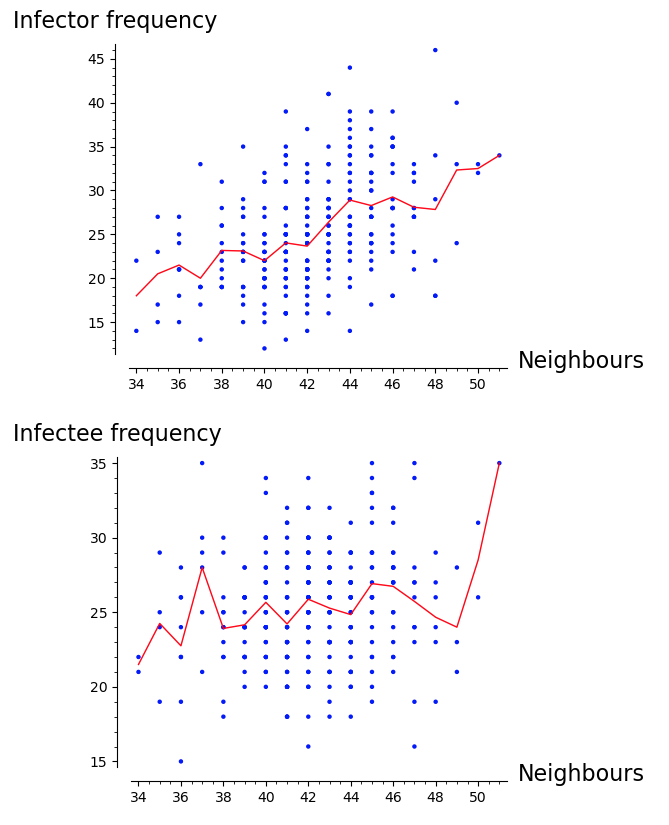
\includegraphics[scale=0.7]{sissmallworld.png}   
    \caption{Infector/infectee frequency for a 15000-event simulation on a small-world network with $n=300$, $k=30$ and $p=0.4$ using the SIS-model.}
    \label{SWresultplot}
\end{figure}
\FloatBarrier
\section{Discussion}
We give a stochastic description of the transmission process on networks in Section \ref{section1} using probability theory and Markov chains. We see how the transmission tree and the deterministic networks are constructed in Section \ref{tree-section}. In \ref{simulation-section}, we see how the parameter $\lambda_2$ affect simulations on networks using the SIR- and SIS-models. As expected, higher values of $\lambda_2$ increase the chances of a recovery event, and so the virus dies out faster for all networks. In \ref{smallsection}, we see how a small world is constructed and how the number of neighbours affects the infector/infectee frequency. The infector/infectee frequency is positively correlated to a node's number of neighbours.

There is a fourth model not considered in this report; the SIRS-model (susceptible-infected-recovered-susceptible). This effectively combines the SIR- and SIS-models into something more complex. The model is not considered because of time-constraints. The SIRS-model does not come with any new behaviour which is not present in the other models, but we shall briefly describe anyway, similar to Section \ref{SIR-model-section} and \ref{sis-model-section}. 

Let infections happen at a rate $\lambda_1$, recoveries at a rate $\lambda_2$ and let recovered nodes turn susceptible (a so-called susceptibility event) at a rate $\lambda_3$. For smaller $\lambda_3$, the nodes stay recovered for longer on average, and the infection will have a hard time spreading. If $\lambda_3$ is larger, recovered nodes turn susceptible faster and this helps the virus staying alive. An SIS-model is a simply an SIRS-model with $\lambda_3 \rightarrow \infty$. There are now three different events that can happen at each step; an infection, a recovery, or a susceptibility event. Let $n_z^{(r)}$ be the number of recovered nodes at event z. Then,
\begin{equation}\label{SIRS-P1}
    P(\text{Event z+1 is an infection event}) := \delta_z = \frac{n^{(c)}_z\lambda_1}{n^{(c)}_z\lambda_1+n^{(i)}_z\lambda_2+n_z^{(r)}\lambda_3},
\end{equation}
\begin{equation}\label{SIRS-P2}
    P(\text{Event z+1 is a recovery event}) := \Delta_z = \frac{n^{(i)}_z\lambda_2}{n^{(c)}_z\lambda_1+n^{(i)}_z\lambda_2+n_z^{(r)}\lambda_3},
\end{equation}
\begin{equation}\label{SIRS-P3}
    P(\text{Event z+1 is a susceptibility event}) := 1-\delta_z-\Delta_z.
\end{equation}

Let $\mathbb{I}$ and $\mathbb{R}$ and $\mathbb{S}$ be defined as in the mathematical preliminaries (Section \ref{prelim}). The transition probability is then
\begin{equation} \label{firstPSIRS}
\begin{split}
P(X(z+1) = x' |X(z)= x) =
\begin{cases}
& \frac{\delta_z}{n_z^{(c)}}  \quad \text{if} \quad x' \in \mathbb{I}(x) \\
& \frac{\Delta_z}{n_z^{(i)}}  \quad \text{if} \quad x' \in \mathbb{R}(x) \\
& \frac{1-\delta_z-\Delta_z}{n_z^{(r)}}  \quad \text{if} \quad x' \in \mathbb{S}(x) \\
& 0 \quad \text{otherwise,}
\end{cases}
\end{split}
\end{equation}
The generator for the Markov process is
\begin{equation}\label{qSIRS}
    q(x(z)\Rightarrow x') = 
    \begin{cases}
    & \lambda_1 \quad \text{if} \quad x' \in \mathbb{I}(x(z)) \\
    & \lambda_2 \quad \text{if} \quad x' \in \mathbb{R}(x(z)) \\
    & \lambda_3 \quad \text{if} \quad x' \in \mathbb{S}(x(z)) \\
    & -\lambda_1n_z^{(c)}-\lambda_2n_z^{(i)}-\lambda_3n_z^{(r)}   \quad \text{if} \quad x' = x(z)\\
    & 0 \quad \text{otherwise.}
    \end{cases}
\end{equation}

For low values of $\lambda_3$ recovered nodes take very long time to turn susceptible, which causes the states to oscillate slowly enough for the model to act as an SIR-model. If $\lambda_3$ is very large, recovered nodes turn susceptible very quickly, which causes this model to act remarkably similar to the SIS-model. When $\lambda_3$ is moderately large, the model yields new interactions and behaviour that might interest the reader enough for them to try their own simulations.

The code openly available at \cite{github} can simulate transmission on an arbitrary network using the SIRS model using $$SIRS(C,lambda1,lambda2,lambda3,z_{end} = 3000,plt=1).$$
The three commands \textit{SIS, SIR} and \textit{SIRS} in the code are dummy functions calling the same parent function named \textit{transmissionProcess}. This function have another parameter called $p_b$ which is a number between 0 and 1. As a susceptible node turns infected, each of its connections has a probability $p_b$ of being \textit{blocked}, which simulate people going into isolation as they become sick.

\bibliography{bibliography}{}
\bibliographystyle{vancouver}
\end{document}
